\documentclass{article}

% if you need to pass options to natbib, use, e.g.:
\PassOptionsToPackage{sort&compress,numbers}{natbib}
% before loading nips_2017
%
% to avoid loading the natbib package, add option nonatbib:
% \usepackage[nonatbib]{nips_2017}

% \usepackage{nips_2017}
% \usepackage[final]{nips_2017}

% to compile a camera-ready version, add the [final] option, e.g.:
\usepackage[final]{nips_2017}

\usepackage[utf8]{inputenc} % allow utf-8 input
\usepackage[T1]{fontenc}    % use 8-bit T1 fonts
\usepackage{hyperref}       % hyperlinks
\usepackage{url}            % simple URL typesetting
\usepackage{booktabs}       % professional-quality tables
\usepackage{amsfonts}       % blackboard math symbols
\usepackage{nicefrac}       % compact symbols for 1/2, etc.
\usepackage{microtype}      % microtypography
\usepackage[pdftex]{graphicx}
\usepackage{dsfont}
\usepackage{subcaption}
\usepackage{amsmath}
\usepackage{amssymb}
\usepackage{xspace}
\usepackage{enumitem}

% \usepackage[sort]{cite}

% additional definitions
\usepackage{color}
\definecolor{darkred}{RGB}{180,50,20}
\definecolor{darkgreen}{RGB}{20,180,50}
\definecolor{purple}{RGB}{90,20,90}
\definecolor{fr}{RGB}{60,125,161}
\newcommand{\ow}[1] {\emph{\textcolor{darkred}{OW: #1}}}
\newcommand{\es}[1] {\emph{\textcolor{darkgreen}{ES: #1}}}
\newcommand{\td}[1] {\emph{\textcolor{purple}{TD: #1}}}
\newcommand{\deepak}[1] {\emph{\textcolor{darkred}{DP: #1}}}
\newcommand{\rz}[1] {\emph{\textcolor{fr}{rz: #1}}}
%\setlength\abovedisplayskip{10pt}


\newcommand{\pp}{\texttt{pix2pix}\xspace}
\newcommand{\ppn}{\texttt{pix2pix+noise}\xspace}
\newcommand{\cinfogan}{\texttt{cLR-GAN}\xspace}
\newcommand{\cae}{\texttt{cAE-GAN}\xspace}
\newcommand{\cvaegan}{\texttt{cVAE-GAN}\xspace}
\newcommand{\cvaeganp}{\texttt{cVAE-GAN++}\xspace}
\newcommand{\bicycle}{\texttt{BicycleGAN}\xspace} %cVAE-LR-GAN
\newcommand{\G}{G\xspace}
\newcommand{\D}{D\xspace}
\newcommand{\E}{E\xspace}
\newcommand{\A}{\mathbf{A}\xspace}
\newcommand{\B}{\mathbf{B}\xspace}
\newcommand{\Bh}{\widehat{\mathbf{B}}\xspace}
\newcommand{\z}{\mathbf{z}\xspace}
\newcommand{\zh}{\widehat{\mathbf{z}}\xspace}
% \newcommand{\L}{\mathcal{L}\xspace}
\newif\ifsubmit
\submitfalse

\ifsubmit
\newcommand{\jy}[1]{}
\newcommand{\revjy}[1]{}
\else
\newcommand{\jy}[1]{\textcolor{blue}{JY: #1}}
\newcommand{\revjy}[1]{\textcolor{blue}{#1}}
\fi


% Papers may be only up to 8 pages long, including figures. An additional ninth page containing only cited references and acknowledgments is allowed. Papers that exceed 9 pages will be rejected without review.

% \usepackage{fancyhdr}
% \usepackage{pdfpages}
% \pagestyle{fancy}
% \fancyhf{}
% \fancyhead[C]{\textbf{DRAFT - Please do not distribute}}
% \fancyfoot[C]{\thepage}


\title{Toward Multimodal Image-to-Image Translation}


% The \author macro works with any number of authors. There are two
% commands used to separate the names and addresses of multiple
% authors: \And and \AND.
%
% Using \And between authors leaves it to LaTeX to determine where to
% break the lines. Using \AND forces a line break at that point. So,
% if LaTeX puts 3 of 4 authors names on the first line, and the last
% on the second line, try using \AND instead of \And before the third
% author name.


\author{
  Jun-Yan Zhu\\
  UC Berkeley\\
%   \texttt{\{junyanz,rich.zhang,pathak\}@eecs.berkeley.edu} \\
  \And
  Richard Zhang\\
  UC Berkeley\\
  \And
  Deepak Pathak\\
  UC Berkeley\\
  \AND
  Trevor Darrell\\
  UC Berkeley\\
  \And
    Alexei A. Efros\\
    UC Berkeley\\
%   \texttt{\{trevor,efros\}@eecs.berkeley.edu} \\
  \And
  Oliver Wang\\
  Adobe Research\\
  \And
  Eli Shechtman\\
  Adobe Research\\
%   \texttt{\{elishe,owang\}@adobe.com} \\
}


\begin{document}
% \nipsfinalcopy is no longer used

\maketitle

\begin{abstract}
We introduce Causal Diffusion as the autoregressive (AR) counterpart of Diffusion models. It is a next-token(s) forecasting framework that is friendly to both discrete and continuous modalities and compatible with existing next-token prediction models like LLaMA and GPT. While recent works attempt to combine diffusion with AR models, we show that introducing sequential factorization to a diffusion model can substantially improve its performance and enables a smooth transition between AR and diffusion generation modes. Hence, we propose \textbf{CausalFusion} - a decoder-only transformer that dual-factorizes data across sequential tokens and diffusion noise levels, leading to state-of-the-art results on the ImageNet generation benchmark while also enjoying the AR advantage of generating an arbitrary number of tokens for in-context reasoning. We further demonstrate CausalFusion's multimodal capabilities through a joint image generation and captioning model, and showcase CausalFusion's ability for zero-shot in-context image manipulations. We hope that this work could provide the community with a fresh perspective on training multimodal models over discrete and continuous data.
\end{abstract}

\vspace{-10pt}
\section{Introduction}
\label{sec:intro}
Autoregressive (AR) and diffusion models are two powerful paradigms for data distribution modeling. AR models, also known as the next token prediction approach, dominate language modeling and are considered central to the success of large language models (LLMs)~\cite{gpt1,gpt2,gpt3,llama1,llama2,llama3}. On the other hand, diffusion models~\cite{ddpm,dit,adm,edm}, or score-based generative models~\cite{songscore,lipman2023flow}, have emerged as the leading approach for visual generation, driving unprecedented progress in the era of visual content generation~\cite{sora,rombach2022high,li2023scaling}. 

\begin{figure}[t]
    \centering
    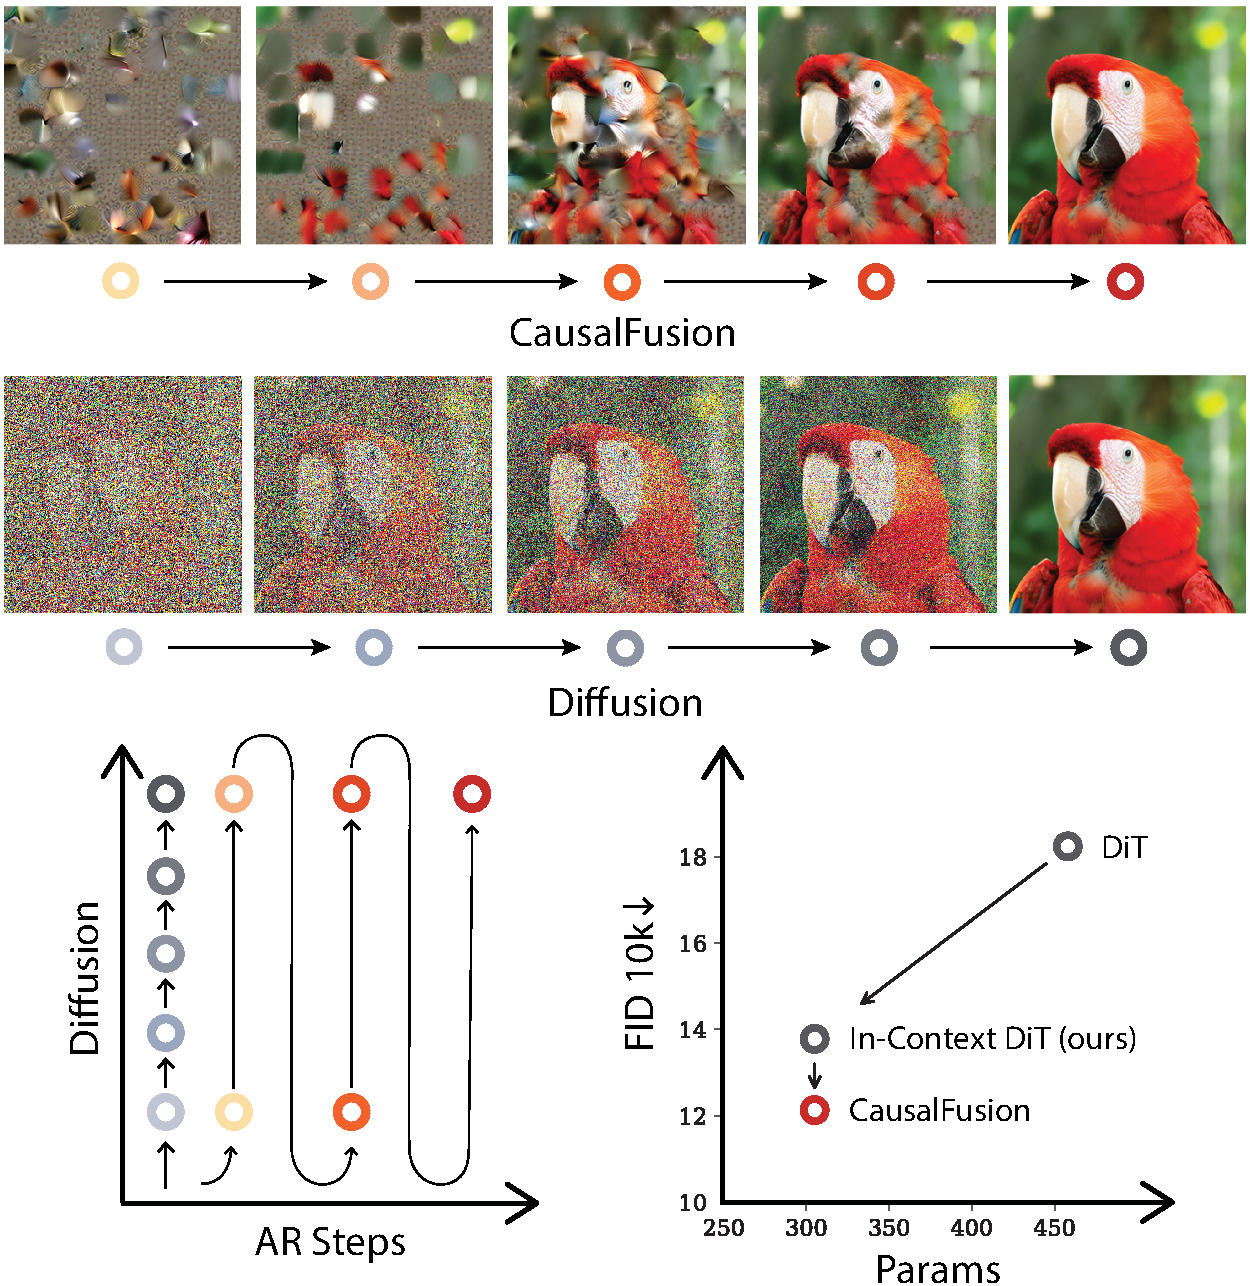
\includegraphics[width=1.0\textwidth,height=1.0\textwidth]{figs/casualfusion-teaser-v6.pdf} 
    \vspace*{-6mm}
    \caption{
    \textbf{Illustration of Dual-Factorization}. The arrow line indicates CausalFusion's generation path, moving from one state to the next by jointly generating along the sequential and noise-level dimension at each step. 
    Compared to DiT, our In-context DiT substantially improves results with fewer parameters. CausalFusion further enhances performance without changing the architecture or parameter count. Results were trained on IN1K for 240 epochs. CausalFusion adopts arbitrary AR steps for image generation, but each step only diffuses partial tokens, resulting in similar (or slightly lower) computational complexity.
    \vspace{-10pt}
    }
    \label{fig:dual-factorization}
\end{figure}


\begin{figure*}[t]
  \centering
  \begin{subfigure}{1.0\linewidth}
    \centering
    \includegraphics[width=\linewidth]{figs/figure2.pdf}
    \caption{Samples generated by CausalFusion-XL/2, ImageNet 512$\times$512, 800 epoch, DDPM 250 steps, CFG=4.0}
  \end{subfigure}
  \begin{subfigure}{1.0\linewidth}
    \centering
    \includegraphics[width=\linewidth]{figs/edit.pdf}
    \caption{\textbf{Zero-shot image editing} results generated by CausalFusion-XL/2, ImageNet 512$\times$512, 800 epoch. We first generate the original image (those on the left), then mask out its centre region, top-half, or bottom-half, and regenerate the image with new class conditions. Details are discussed in Sec \ref{sec:system}.}
  \end{subfigure}
  \caption{\textbf{Visualization results}. All samples are generated by models trained only on \textbf{ImageNet-1K class-conditional generation} task, demonstrating CausalFusion's zero-shot image manipulation ability. See more visualization results in Appendix~\ref{appendix:secD}.
  \vspace{-12pt}
  }
  \vspace{-6pt}
  \label{fig:vis1}
\end{figure*}

The intrinsic distinction between AR and diffusion models lies in their approach to data distribution factorization. AR models treat data as an ordered sequence, factorizing it along the sequential axis, where the probability of each token is conditioned on all preceding tokens. This factorization enables the AR paradigm to generalize effectively and efficiently across arbitrary number of tokens, making it well-suited for long-sequence reasoning and in-context generation. In contrast, diffusion models factorize data along the noise-level axis, where the tokens at each step are a refined (denoised) version of themselves from the previous step. As a result, the diffusion paradigm is generalizable to arbitrary number of data refinement steps, enabling iterative quality improvement with scaled inference compute. While AR and diffusion models each excel within their respective domains, their distinct factorization approaches reveal complementary potential. Although recent studies~\cite{transfusion,monoformer,dart} have attempted to integrate AR and diffusion within a single model, they typically treat these paradigms as separate modes, missing the potential benefits of jointly exploring them within a 2-D factorization plane.

To this end, we introduce \textbf{CausalFusion}, a flexible framework that integrates both sequential and noise-level data factorization to unify their advantages. The degree of factorization along these two axes—namely, the AR step and diffusion step—is adjustable, enabling {CausalFusion} to revert seamlessly to the traditional AR or diffusion paradigms at either extreme. To enhance its generality, CausalFusion is designed to predict \textit{any} number of tokens at \textit{any} AR step, with \textit{any} pre-defined sequence order and \textit{any} level of inference compute, thereby minimizing the inductive biases presented in existing generative models. As shown in Figure~\ref{fig:dual-factorization}, this approach provides a broad spectrum between the AR and diffusion paradigms, allowing smooth interpolation within two endpoints during both training and inference. 
Specifically, we explore CausalFusion in image generation and multimodal generation scenarios, where we observe that the level of training difficulties significantly influences the overall effectiveness of CausalFusion.

\textbf{Difficulties of generative tasks in CausalFusion:} Both AR and diffusion paradigms present unique challenges based on difficulties of their specific generative stages. In diffusion models, the effectiveness of training depends heavily on proper loss weighting across noise levels~\cite{ddpm,minsnr}, as higher noise levels are more difficult and usually provide more valuable signals than lower noise levels. Similarly, AR models are susceptible to error accumulation~\cite{bengio2015scheduled} as early-stage predictions are made with limited visible context, making them more error-prone. Optimizing CausalFusion thus requires balancing across these varying task difficulties to optimize training signal impact and ensure sufficient exploration across the entire factorization plane.

In this paper, we formally examine the difficulties of generative tasks within CausalFusion. We show that, in addition to the noise levels in diffusion and the amount of visible context in AR, the total number of AR steps, which controls the interpolation between AR and diffusion, also plays a critical role in shaping training difficulties. Driven by these factors, we develop a scalable and versatile model based on the CausalFusion framework. Starting from the DiT architecture~\cite{dit}, we gradually convert it into a decoder-only transformer compatible with existing AR models like GPT~\cite{gpt1,gpt2,gpt3} and LLaMA~\cite{llama1,llama2,llama3}. We provide insights on how to appropriately choose the number of AR steps during the training of CausalFusion models, and further introduce loss weighing along both the diffusion and AR axis to balance the impact of different generative stages. As shown in Figure~\ref{fig:dual-factorization} and ~\ref{fig:vis1}, our model achieves state-of-the-art performance on the ImageNet class-conditional generation benchmark, significantly outperforming DiT~\cite{dit} and enabling zero-shot image manipulations due to its AR nature. When pretraining on both text-to-image and image-to-text tasks, our model surpasses forced-fusion frameworks such as TransFusion~\cite{transfusion}, demonstrating the versatility of our CausalFusion framework.


We highlight our main contribution below:
\begin{itemize}
\item  We propose CausalFusion as the AR counterpart to DiT, achieving state-of-the-art results and enabling the unlimited token generation for in-context reasoning.
\item  We systematically study CausalFusion on the dual-factorization plane and identify key factors that improve the effectiveness of CausalFusion models.
\item  Compared with recent studies~\cite{transfusion}, CausalFusion enables a smooth, cohesive integration with language modeling for cross-modal generation and reasoning.
\end{itemize} 


% \begin{figure}[t]
%   \begin{minipage}{0.49\textwidth}
%      \centering
%     \includegraphics[width=1.0\textwidth]{fig/MLMF.png}
%     \caption{Multi-Layer Motion Fusion.}
%     \label{fig: frameselector_abalation}
    
%   \end{minipage}
%   \hfill
%    \begin{minipage}{0.48\textwidth}
%     \centering
%     \includegraphics[width=0.8\textwidth]{fig/SMPL.jpg}
%     \caption{Prametric Shape Alignment.}
%     \label{fig:Visualizedselected_frames}
%   \end{minipage}
% \vspace{-3mm}
% \end{figure}


\section{Related Work}
\label{sec:related_work}

\textbf{Diffusion Models for Image Generation.}
Diffusion-based models~\cite{balaji2022ediffi,huang2023composer,nichol2021glide,ramesh2022hierarchical,rombach2022high,saharia2022photorealistic} have rapidly emerged as a fundamental component in the domain of text-to-image generation, renowned for their capacity to yield highly promising generative outcomes. 
To address the considerable computational requirements inherent in diffusion models, the Latent Diffusion Model, as proposed in~\cite{rombach2022high} introduces a technique for denoising within the latent space.
This method not only enhances the computational efficiency of these models but also preserves their ability to generate high-fidelity images.
Moreover, in the endeavor to enhance control over visual generation, recent studies such as ControlNet~\cite{zhang2023adding}, T2I-Adapter~\cite{mou2023t2i}, and IP-Adapter~\cite{ye2023ip} have delved into the incorporation of supplementary encoder layers.
These layers facilitate the assimilation of control signals encompassing aspects such as pose, depth, and edge information, and even permit the utilization of images in conjunction with textual prompts.
This progression signifies a significant advancement towards more controlled and precise image generation, facilitating the creation of images characterized by not only superior quality but also enriched contextual accuracy and detail.


\textbf{Diffusion Models for Human Image Animation.}
The task of animating human images, a significant endeavor within the domain of video generation, aims to seamlessly create videos from one or multiple static images~\cite{chan2019everybody,ren2020deep,siarohin2019first,siarohin2021motion,yu2023bidirectionally,zhang2022exploring,zhao2022thin,yoon2021pose, sarkar2021neural, hu2023sherf, albahar2023humansgd, cao2023dreamavatar, prokudin2021smplpix, fu2022styleganhuman, jiang2023humangen}.
The recent advancements of diffusion models in the text-to-image domain have sparked interest in exploring their utility for animating human images.
PIDM~\cite{bhunia2023person} introduces a texture diffusion module that is specifically crafted to align the texture patterns of the source and target images closely, thereby enhancing the realism of the resultant animated output.
DreamPose~\cite{karras2023dreampose} capitalizes on the capabilities of the pre-trained Stable Diffusion model by incorporating both CLIP~\cite{radford2021learning} and VAE~\cite{kingma2013auto} for image encoding. 
It integrates these embeddings with an adapter. 
Similarly, DisCo~\cite{wang2023disco} innovatively segregates the control of pose and background using dual independent ControlNets~\cite{zhang2023adding}, providing finer control over the animation process. 
Animate Anyone~\cite{hu2023animate} utilizes a UNet-based ReferenceNet to extract features from reference images.
It includes pose information via a lightweight pose guider. Expanding on the principles introduced by AnimateDiff~\cite{guo2023animatediff}, Animate Anyone integrates a temporal layer into the denoising UNet to enhance temporal coherence.
MagicAnimate~\cite{xu2023magicanimate} follows a similar approach but employs a ControlNet tailored for DensePose \cite{guler2018dense} inputs instead of the more commonly used OpenPose~\cite{cao2017realtime} keypoints to provide more precise pose guidance.
This paper primarily builds upon esteemed diffusion-based methodologies and advances the optimization of appearance alignment and motion guidance mechanisms. 
This is achieved by introducing a 3D parametric model for geometric reconstruction of the reference image and motion modeling of the source video sequence.


\textbf{Pose Guidance in Human Image Animation.}
DWpose\cite{yang2023effective} stands out as an enhanced alternative to OpenPose\cite{cao2017realtime}, offering more accurate and expressive skeletons. 
This improvement has proven beneficial for diffusion models in generating higher quality images, with its adoption as a condition signal in various works\cite{feng2023dreamoving,hu2023animate}.
The work presented in DensePose~\cite{Guler2018DensePose} aims to establish dense correspondences between an RGB image and a surface-based representation.
The SMPL~\cite{SMPL:2015} model is a 3D model renowned for its realistic depiction of human bodies through skinning and blend shapes.
Its widespread adoption spans fields like human reconstruction\cite{he2021arch,alldieck2018video} and interaction with environments\cite{hassan2021populating,ma2020learning}. 
It also serves as essential ground truth for neural networks in pose and shape analysis\cite{lu2023dposer,mu2023actorsnerf}.
In this paper, we consider SMPL, the 3D parametric model, to reconstruct the poses as well as the shapes from the source video, and obtain more complete condition for appearance alignment and pose guidance.

\begin{figure}[t]
  \centering
  \includegraphics[width=0.95\linewidth]{fig/framework.jpg}
  \caption{The overview of our proposed approach. Given an input human image and a reference video depicting a motion sequence. We obtain the pose sequence corresponding to the reference image through Parametric Shape Alignment as 3D motion guidance. MLMF is employed to encode multi-layer 3D-related motion information. Referencenet and Temporal-attention ensure identity consistency and temporal coherence, respectively.}
  \vspace{-6mm}
  \label{fig:network}
\end{figure}

\section{Multimodal Image-to-Image Translation}
\label{sec:methods}
Our goal is to learn a multi-modal mapping between two image domains, for example, edges and photographs, or night and day images, etc. 
Consider the input domain $\mathcal{A}\!\subset\!\mathds{R}^{H\!\times W\!\times 3}$, which is to be mapped to an output domain $\mathcal{B}\!\subset\!\mathds{R}^{H\!\times W\!\times 3}$. 
During training, we are given a dataset of paired instances from these domains, $\big\{(\A\!\in\!\mathcal{A}, \B\!\in\!\mathcal{B})\big\}$, which is representative of a joint distribution $p(\A,\B)$.
It is important to note that there could be multiple plausible paired instances $\B$ that would correspond to an input instance $\A$, but the training dataset usually contains only one such pair.
However, given a new instance $\A$ during test time, our model should be able to generate a diverse set of output $\Bh$'s, corresponding to different modes in the distribution $p(\B|\A)$.

While conditional GANs have achieved success in image-to-image translation tasks~\citep{pathakCVPR16context,sangkloy2017scribbler,xian2017texturegan,yang2016high,isola2016image,zhu2017unpaired}, they are primarily limited to generating a deterministic output $\Bh$ given the input image $\A$. 
On the other hand, we would like to learn the mapping that could sample the output $\Bh$ from true conditional distribution given $\A$, and produce results which are both diverse and realistic.
To do so, we learn a low-dimensional latent space $\z \in \mathds{R}^{Z}$, which encapsulates the ambiguous aspects of the output mode which are not present in the input image. For example, a sketch of a shoe could map to a variety of colors and textures, which could get compressed in this latent code. We then learn a deterministic mapping $\G:(\A,\z)\rightarrow \B$ to the output. To enable stochastic sampling, we desire the latent code vector $\z$ to be drawn from some prior distribution $p(\z)$; we use a standard Gaussian distribution $\mathcal{N}(0,I)$ in this work.

We first discuss a simple extension of existing methods and discuss its strengths and weakness, motivating the development of our proposed approach in the subsequent subsections.

\subsection{Baseline: \ppn ($\z \rightarrow \Bh$)}
The recently proposed \pp model~\citep{isola2016image} has shown high quality results in the image-to-image translation setting.
It uses conditional adversarial networks~\citep{goodfellow2014generative,mirza2014conditional} to help produce perceptually realistic results. GANs train a generator $\G$ and discriminator $\D$ by formulating their objective as an adversarial game. The discriminator attempts to differentiate between real images from the dataset and fake samples produced by the generator. Randomly drawn noise $\z$ is added to attempt to induce stochasticity.
We illustrate the formulation in Figure \ref{fig:fig2}(b) and describe it below.
\begin{equation}
\mathcal{L}_{\text{GAN}}(\G,\D) = \mathds{E}_{\A,\B\sim p(\A,\B)}[\log(\D(\A,\B))] + \mathds{E}_{\A\sim p(\A),\z\sim p(\z)}[ \log(1-\D(\A,\G(\A,\z)))]
\label{eqn:Lgan}
\end{equation}

To encourage the output of the generator to match the input as well as stabilize the training, we use an $\ell_1$ loss between the output and the ground truth image.
\begin{equation}
\mathcal{L}_{1}^{\text{image}}(\G) = \mathds{E}_{\A,\B\sim p(\A,\B),\z\sim p(\z)} ||\B - \G(\A,\z) ||_1
\label{eqn:L1}
\end{equation}

The final loss function uses the GAN and $\ell_1$ terms, balanced by $\lambda$. 
\begin{equation}
\G^{*} = \arg\min_{\G} \max_{\D} \quad \mathcal{L}_{\text{GAN}}(\G,\D) + \lambda \mathcal{L}_1^{\text{image}}(\G)
\end{equation}

In this scenario, there is little incentive for the generator to make use of the noise vector which encodes random information.
Isola et al.~\citep{isola2016image} note that the noise was ignored by the generator in preliminary experiments and was removed from the final experiments.
This was consistent with observations made in the conditional settings by~\citep{pathakCVPR16context,mathieu2015deep}, as well as the mode collapse phenomenon observed in unconditional cases~\citep{salimans2016improved,goodfellow2016nips}.
In this paper, we explore different ways to explicitly enforce
%the generator to use the latent encoding, by making it
the latent coding to
capture relevant information.

\subsection{Conditional Variational Autoencoder GAN: \cvaegan ($\B \rightarrow \z \rightarrow \widehat{\mathbf{B}}$)}
One way to force the latent code $\z$ to be ``useful" is to directly map the ground truth $\B$ to it using an encoding function $\E$.
The generator $\G$ then uses both the latent code and the input image $\A$ to synthesize the desired output $\widehat{\mathbf{B}}$.
The overall model can be easily understood as the reconstruction of $\B$, with latent encoding $\z$ concatenated with the paired $\A$ in the middle -- similar to an autoencoder~\citep{hinton2006reducing}. This interpretation is better shown in Figure \ref{fig:fig2}(c).

This approach has been successfully investigated in Variational Autoencoder~\citep{kingma2013auto} in the unconditional scenario without the adversarial objective. Extending it to conditional scenario, the distribution $Q(\z|\B)$ of latent code $\z$ using the encoder $\E$ with a Gaussian assumption, $Q(\z|\B)\triangleq\E(\B)$. To reflect this, Equation \ref{eqn:Lgan} is modified to sampling $\z\sim\E(\B)$ using the re-parameterization trick, allowing direct back-propagation~\citep{kingma2013auto}. 
\begin{equation}
\mathcal{L}_{\text{GAN}}^{\text{VAE}} = \mathds{E}_{\A,\B\sim p(\A,\B)}[\log(\D(\A,\B))] + \mathds{E}_{\A,\B\sim p(\A,\B),\z\sim E(\B)}[ \log(1-\D(\A,\G(\A,\z)))]
\label{eqn:LVAE}
\end{equation}
We make the corresponding change in the $\ell_1$ loss term in Equation \ref{eqn:L1} as well to obtain $\mathcal{L}_1^{\text{VAE}}(\G)=\mathds{E}_{\A,\B\sim p(\A,\B),\z\sim \E(\B)} ||\B - \G(\A,\z) ||_1$. Further, the latent distribution encoded by $E(B)$ is encouraged to be close to a random Gaussian to enable sampling at inference time, when $\B$ is not known.
\begin{equation}
\mathcal{L}_{\text{KL}}(\E) = \mathds{E}_{\B\sim p(\B)} [ \mathcal{D}_{\text{KL}}(\E(\B) || \;\mathcal{N}(0,I)) ],
\label{eqn:KL}
\end{equation}
where $\mathcal{D}_{\text{KL}}(p||q)=-\int  p(z) \log\frac{p(z)}{q(z)}dz $. This forms our \cvaegan objective, a conditional version of the VAE-GAN~\citep{larsen2016vaegan} as
\begin{equation}
\G^{*}, \E^{*} = \arg\min_{\G,\E} \max_{\D}  \quad \mathcal{L}_{\text{GAN}}^{\text{VAE}}(\G,\D,\E)
+ \lambda\mathcal{L}_1^{\text{VAE}}(\G, \E)+\lambda_{\text{KL}}\mathcal{L}_{\text{KL}}(\E).
\end{equation}

As a baseline, we also consider the deterministic version of this approach, i.e., dropping KL-divergence and encoding $\z=E(\B)$.
We call it \cae and show a comparison in the experiments.
There is no guarantee in \cae on the distribution of the latent space $\z$, which makes the test-time sampling of $\z$ difficult. 

% cite cvae-gan
\subsection{Conditional Latent Regressor GAN: \cinfogan ($\z \rightarrow \Bh \rightarrow \zh$)}
We explore another method of enforcing the generator network to utilize the latent code embedding $\z$, while staying close to the actual test time distribution $p(\z)$, but from the latent code's perspective.
As shown in Figure \ref{fig:fig2}(d), we start from a 
% randomly drawn latent code $\z$ and enforce $\E(\G(\A,\z))$ to map back to the same latent code,
randomly drawn latent code $\z$ and attempt to recover it with $\zh=\E(\G(\A,\z))$.
% using an $\ell_1$ loss.
Note that the encoder $\E$ here is producing a point estimate for $\zh$, whereas the encoder in the previous section was predicting a Gaussian distribution.
\begin{equation}
\mathcal{L}_{1}^{\text{latent}}(\G,\E) = \mathds{E}_{\A\sim p(\A),\z\sim p(\z)} ||\z - \E(\G(\A,\z)) ||_1
\label{eqn:L1_lacyc}
\end{equation}

We also include the discriminator loss $L_{\text{GAN}}(\G,\D)$ (Equation \ref{eqn:Lgan}) on $\Bh$ to encourage the network to generate realistic results, and the full loss can be written as:
\begin{equation}
\G^{*}, \E^{*} = \arg\min_{\G,\E} \max_\D \quad \mathcal{L}_{\text{GAN}}(\G,\D) + \lambda_{\text{latent}} \mathcal{L}_1^{\text{latent}}(\G,\E)
\label{fig:L}
\end{equation}

The $\ell_1$ loss for the ground truth image $\B$ is not used. Since the noise vector is randomly drawn, the predicted $\Bh$ does not necessarily need to be close to the ground truth but does need to be realistic. The above objective bears similarity to the ``latent regressor" model~\citep{donahue2016adversarial,dumoulin2016adversarially,xi2016infogan}, where the generated sample $\Bh$ is encoded to generate a latent vector.

\subsection{Our Hybrid Model: \bicycle}
\label{sec:finalMethod}
We combine the \cvaegan and \cinfogan objectives in a hybrid model. For \cvaegan, the encoding is learned from real data, but a random latent code may not yield realistic images at test time -- the KL loss may not be well optimized. Perhaps more importantly, the adversarial classifier $\D$ does not have a chance to see results sampled from the prior during training. 
%  latent space may not be organized in an easy manner to be sampled from
In \cinfogan, the latent space is easily sampled from a simple distribution, but the generator is trained without the benefit of seeing ground truth input-output pairs. We propose to train with constraints in both directions, aiming to take advantage of both cycles ($\B \rightarrow \z \rightarrow \widehat{\mathbf{B}}$ and $\z \rightarrow \Bh \rightarrow \zh$), hence the name \bicycle.

\vspace{-3mm}
\begin{equation}
\begin{split}
\G^{*}, \E^{*} = \arg\min_{\G,\E} \max_{\D} \quad  & \mathcal{L}_{\text{GAN}}^{\text{VAE}}(\G,\D,\E) + \lambda \mathcal{L}_1^{\text{VAE}}(\G,\E) \\
+& \mathcal{L}_{\text{GAN}}(\G,\D) + \lambda_{\text{latent}} \mathcal{L}_1^{\text{latent}}(\G,\E) + \lambda_{\text{KL}}\mathcal{L}_{\text{KL}}(\E),
\end{split}
\label{eq:L}
\end{equation}
where the hyper-parameters $\lambda$, $\lambda_{\text{latent}}$, and $\lambda_{\text{KL}}$ control the relative importance of each term. 

In the unconditional GAN setting, \citet{larsen2016vaegan} observe that using samples from both the prior $\mathcal{N}(0,I)$ and encoded $\E(\B)$ distributions further improves results.
Hence, we also report one variant which is the full objective shown above (Equation~\ref{eq:L}), but without the reconstruction loss on the latent space $\mathcal{L}_1^{\text{latent}}$. 
We call it \cvaeganp, as it is based on \cvaegan with an additional loss $\mathcal{L}_{\text{GAN}}(G, D)$, which allows the discriminator to see randomly drawn samples from the prior.
\vspace{-2mm}

\section{Implementation Details}
\label{sec:implementation}
The code and additional results are publicly available at \url{https://github.com/junyanz/BicycleGAN}. Please refer to our website for more details about the datasets, architectures, and training procedures.
\begin{figure}
\centering
% \hspace{-.08\linewidth}
\includegraphics[width=1.0\linewidth]{imgs/injectz.pdf}
\caption{\small \textbf{Alternatives for injecting {\bf z} into generator.} Latent code \textbf{z} is injected by spatial replication and concatenation into the generator network. We tried two alternatives, {\bf (left)} injecting into the input layer and {\bf (right)} every intermediate layer in the encoder.}
\vspace{-4mm}
\label{fig:addz}
\end{figure}

\paragraph{Network architecture} For generator $\G$, we use the U-Net~\citep{ronneberger2015u}, which contains an encoder-decoder architecture, with symmetric skip connections. The architecture has been shown to produce strong results in the unimodal image prediction setting when there is a spatial correspondence between input and output pairs. For discriminator $\D$, we use two PatchGAN discriminators~\citep{isola2016image} at different scales, which aims to predict real vs. fake for $70\times 70$ and $140 \times 140$ overlapping image patches. For the encoder $\E$, we experiment with two networks: (1) \texttt{E\textsubscript{CNN}}: CNN with a few convolutional and downsampling layers and (2) \texttt{E\textsubscript{ResNet}}: a classifier with several residual blocks~\cite{he2016deep}.

\paragraph{Training details} We build our model on the Least Squares GANs (LSGANs) variant~\citep{mao2016least}, which uses a least-squares objective instead of a cross entropy loss. LSGANs produce high-quality results with stable training. We also find that not conditioning the discriminator $\D$ on input $\mathbf{A}$ leads to better results (also discussed in~\citep{pathakCVPR16context}), and hence choose to do the same for all methods. We set the parameters $\lambda_{\text{image}}=10$, $\lambda_{\text{latent}}=0.5$ and $\lambda_{\text{KL}}=0.01$ in all our experiments. We tie the weights for the generators and encoders in the \cvaegan and \cinfogan models. For the encoder, only the predicted mean is used in \cinfogan. We observe that using two separate discriminators yields slightly better visual results compared to sharing weights. We only update $\G$ for the $\ell_1$ loss $\mathcal{L}_{1}^{\text{latent}}(\G,\E)$ on the latent code (Equation \ref{eqn:L1_lacyc}), while keeping $\E$ fixed. We found optimizing $\G$ and $\E$ simultaneously for the loss would encourage $G$ and $E$ to hide the information of the latent code without learning meaningful modes.
We train our networks from scratch using Adam~\citep{kingma2014adam} with a batch size of $1$ and with a learning rate of $0.0002$. We choose latent dimension $|\z|=8$ across all the datasets. 

{\bf Injecting the latent code $\z$ to generator}.
We explore two ways of propagating the latent code $\z$ to the output, as shown in Figure~\ref{fig:addz}: 
(1) \texttt{add\_to\_input}: we spatially replicate a $Z$-dimensional latent code $\z$ to an $H\!\times W\!\times Z$ tensor and concatenate it with the $H\!\times W\!\times 3$ input image and (2)~\texttt{add\_to\_all}: we add $\z$ to each intermediate layer of the network $\G$, after spatial replication to the appropriate sizes.

\vspace{-1mm}

\section{Experiments}

\begin{figure}[tb]
  \centering
  %
  \begin{subfigure}{0.31\linewidth}
  \includegraphics[width=\linewidth]{images/closeup/khady_gt_22_detail.png}
  \includegraphics[width=\linewidth]{images/closeup/kitten_gt_67_detail.png}
  \includegraphics[width=\linewidth]{images/closeup/pug_gt_25_detail.png}
  \caption{Ground Truth Image}
  \end{subfigure}
  %
  \hfill
  %
  \begin{subfigure}{0.31\linewidth}
  \includegraphics[width=\linewidth]{images/closeup/khady_3dgs_22_detail.png}
  \includegraphics[width=\linewidth]{images/closeup/kitten_3dgs_67_detail.png}
  \includegraphics[width=\linewidth]{images/closeup/pug_3dgs_25_detail.png}
  \caption{3DGS~\cite{kerbl3Dgaussians}}
  \end{subfigure}
  %
  \hfill
  %
  \begin{subfigure}{0.31\linewidth}
  \includegraphics[width=\linewidth]{images/closeup/khady_rgb_22_detail.png}
  \includegraphics[width=\linewidth]{images/closeup/kitten_rgb_67_detail.png}
  \includegraphics[width=\linewidth]{images/closeup/pug_rgb_25_detail.png}
  \caption*{Frosting (Ours)}
  \end{subfigure}
  %
  \vspace{-0.3cm}
  \caption{
  \textbf{Close-up views of fuzzy materials from the Shelly dataset~\cite{wang-siggraphasia2023-adaptive-shells} reconstructed with vanilla Gaussian Splatting~\cite{kerbl3Dgaussians}~(center) and Frosting~(right).}
  }
  \label{fig:fuzzy-material-closeup}
\end{figure}

\subsection{Implementation Details}


We implemented our method with PyTorch~\cite{paszke-nips19-pytorch} and optimized the representations on a single GPU Nvidia Tesla V100~SXM2~32~Go.
Optimizing a full, editable Frosting model takes between 45 and 90 minutes on a single GPU, depending on the complexity of the scene. This optimization is much faster than the most similar approach to Frosting in the literature, namely Adaptive~Shells~\cite{wang-siggraphasia2023-adaptive-shells}, that requires 8~hours on a single GPU for a synthetic scene, and 1.7 times more iterations for a real scene.

\subsubsection{Extracting the surface mesh.} When reconstructing real scenes, we follow the approach from vanilla 3DGS~\cite{kerbl3Dgaussians} and first use COLMAP to estimate the camera poses and extract a  point cloud for initialization. For synthetic scenes with known camera poses, we just use a random point cloud for initialization. Then, we optimize an unconstrained Gaussian Splatting representation for 7,000 iterations. We save these Gaussians aside and apply the regularization term from SuGaR until iteration~15,000. We finally compute an optimal depth parameter $\bar{D}$ with $\gamma=100$ and extract a mesh from the regularized Gaussians by applying Poisson surface reconstruction as described in~\cite{guedon2023sugar}.

\subsubsection{Optimizing the Gaussian Frosting.} Given a budget of $N$ Gaussians, we initialize $N$ Gaussians in the Frosting layer and optimize them for 15,000 additional iterations, which gives a total of 30,000 iterations, similarly to 3DGS~\cite{kerbl3Dgaussians}. Vanilla 3DGS optimization generally produces between 1 and 5 million Gaussians. In practice, we use $N$=5~million for real scenes and $N$=2~million for synthetic scenes.


\subsection{Real-Time Rendering in Complex Scenes}

To evaluate the quality of Frosting's rendering, we compute the standard metrics PSNR, SSIM and LPIPS~\cite{zhang-2018-cvpr-lpips} and compare to several baselines, some of them focusing only on Novel View Synthesis~\cite{mildenhall2020nerf,wang2021neus,barron2021mipnerf,barron2022mipnerf360,mueller2022instantngp,yu_and_fridovichkeil2021plenoxels,kerbl3Dgaussians} and others relying on an editable representation~\cite{chen2022mobilenerf,rakotosaona2023nerfmeshing,yariv-2023-bakedsdf,reiser2024binaryopacitygrid,wang-siggraphasia2023-adaptive-shells,guedon2023sugar}, just like Frosting. We compute metrics on several challenging datasets containing synthetic and real scenes.\\

\noindent
\textbf{Shelly.} We first compare Frosting to state-of-the-art methods on the dataset Shelly introduced in Adaptive~Shells~\cite{wang-siggraphasia2023-adaptive-shells}. Shelly includes six synthetic scenes with challenging fuzzy materials that surface-based approaches struggle to reconstruct accurately. As we show in Table~\ref{tab:nvsmetrics_shelly} and Figure~\ref{fig:fuzzy-material-closeup}, Frosting outperforms every other methods for all three metrics. Frosting even outperforms with a wide margin vanilla Gaussian Splatting, which is free from any surface constraints and only focuses on optimizing the rendering quality. Indeed, the sampling of Gaussians inside the Frosting layer provides a much more efficient densification of Gaussians than the strategy proposed in 3DGS~\cite{kerbl3Dgaussians}, targeting the challenging fuzzy areas close to the surface and allocating more Gaussians where volumetric rendering is needed.\\

\noindent
\textbf{NeRFSynthetic.} Table~\ref{tab:nvsmetrics_shelly} provides a comparison on the NeRFSynthetic data\-set~\cite{mildenhall2020nerf}, which consists in eight synthetic scenes. Frosting performs the best among the editable methods, surpassing Su\-GaR~\cite{guedon2023sugar}, and achieves results on par with vanilla 3DGS and other radiance field methods.\\

\begin{table}
   \caption{
   \antoine{
   \textbf{Quantitative evaluation of rendering quality on the synthetic datasets \emph{Shelly}~\cite{wang-siggraphasia2023-adaptive-shells} and \emph{NeRFSynthetic}~\cite{mildenhall2020nerf}.} Frosting is the best among all methods, outperforming even non-editable models that only focus on rendering. Contrary to an unconstrained 3D Gaussian Splatting~\cite{kerbl3Dgaussians}, our representation allows for densifying Gaussians more efficiently by targeting challenging and fuzzy areas.}}
  \label{tab:nvsmetrics_shelly}
  \centering
  {\scriptsize
  \begin{tabular}{@{}lccccccc@{}}
    \toprule
     \multicolumn{1}{c}{} & \multicolumn{3}{c}{\emph{Shelly}} & \multicolumn{3}{c}{\emph{NeRFSynthetic}} \\
     \cmidrule(r){2-4} \cmidrule(r){5-7}
      & PSNR $\uparrow$ & SSIM $\uparrow$ & LPIPS $\downarrow$ & PSNR $\uparrow$ & SSIM $\uparrow$ & LPIPS $\downarrow$ & \\
     %
    %\midrule
    %\multicolumn{4}{l}{\textbf{No mesh (except Frosting)}} \\
    \midrule
    NeRF~\cite{mildenhall2020nerf} & 31.27 & 0.893 & 0.157 & 31.01 & 0.947 & 0.081 & \\
    NeuS~\cite{wang2021neus} & 29.98 & 0.893 & 0.158 & -- & -- & -- & \\
    Mip-NeRF~\cite{barron2021mipnerf}  & 32.59 & 0.899 & 0.148 & \cellcolor{yellow!25}33.09 & 0.961 & 0.043 & \\
    I-NGP~\cite{mueller2022instantngp} & 33.22 & 0.922 & 0.125 & \cellcolor{orange!25}33.18 & -- & -- & \\
    3DGS~\cite{kerbl3Dgaussians}  & \cellcolor{orange!25}37.66 & \cellcolor{orange!25}0.958 & \cellcolor{orange!25}0.066 & \cellcolor{red!25}\textbf{33.32} & \cellcolor{red!25}\textbf{0.970} & \cellcolor{orange!25}0.030 & \\
    \midrule
    MobileNeRF~\cite{chen2022mobilenerf} & 31.62 & 0.911 & 0.129 & 30.90 & 0.947 & 0.062 & \\
    Adaptive Shells~\cite{wang-siggraphasia2023-adaptive-shells}  & 36.02 & \cellcolor{yellow!25}0.954 & 0.079 & 31.84 & 0.957 & 0.056 & \\
    SuGaR\cite{guedon2023sugar}  & \cellcolor{yellow!25}36.33 & \cellcolor{yellow!25}0.954 & \cellcolor{yellow!25}0.059 & 32.40 & \cellcolor{yellow!25}0.964 & \cellcolor{yellow!25}0.033 & \\
    Frosting (Ours)  & \cellcolor{red!25}\textbf{39.84} & \cellcolor{red!25}\textbf{0.977} & \cellcolor{red!25}\textbf{0.033} & 33.03 & \cellcolor{orange!25}0.967 & \cellcolor{red!25}\textbf{0.029} & \\
    \bottomrule
  \end{tabular}
  }
\end{table}

\noindent
\textbf{Mip-NeRF~360.} We also compare Frosting to state-of-the-art approaches on the real scenes from the Mip-NeRF~360 dataset~\cite{barron2022mipnerf360}. This dataset contains images from seven challenging real scenes, but was captured with ideal lighting condition and provides really good camera calibration data and initial SfM~points. Results are available in Table~\ref{tab:nvsmetrics_mipnerf360} and Figure~\ref{fig:frosting-renders}. Frosting reaches the best performance among all editable methods, and obtains worse but competitive results compared to vanilla Gaussian Splatting. When Gaussian Splatting is given a very good initialization with a large amount of SfM points, the benefits from the Gaussian Frosting densification are not as effective, and optimizing Gaussians without additional constraints as in 3DGS slightly improves performance.\\

\noindent
\textbf{Additional real scenes.} We finally compare Frosting to the baselines with captures of real scenes that present variations in exposure or white balance. To this end, we follow the approach from 3DGS~\cite{kerbl3Dgaussians} and select the same two subsets of two scenes from \emph{Tanks\&Temples} (\emph{Truck} and \emph{Train}) and \emph{Deep~Blending}~(\emph{Playroom} and \emph{Dr.~Johnson}). We also evaluate a few methods on a custom dataset that consists of four casual captures made with a smartphone (we call these scenes \emph{SleepyCat}, \emph{Buzz}, \emph{RedPanda}, and \emph{Knight}), illustrated in Figures~\ref{fig:teaser} and~\ref{fig:frosting-renders}. Results are available in Table~\ref{tab:nvsmetrics_tandtdb}. In these more realistic scenarios, Frosting achieves once again similar or better performance than unconstrained Gaussian Splatting even though it is an editable representation that relies on a single, animatable mesh.

\begin{table}
   \caption{\textbf{Quantitative evaluation of rendering quality on the Mip-NeRF~360 dataset~\cite{barron2022mipnerf360}.} \antoine{Frosting is best among the methods that recover an editable Radiance Field with explicit meshes, and achieves performance comparable to NeRF methods and vanilla 3D Gaussian Splatting.} }
  \label{tab:nvsmetrics_mipnerf360}
  \centering
  {\scriptsize
  \begin{tabular}{@{}lcccccccccc@{}}
    \toprule
      %
     \multicolumn{1}{c}{} & \multicolumn{3}{c}{Indoor scenes} & \multicolumn{3}{c}{Outdoor scenes} & \multicolumn{3}{c}{Average on all scenes} \\
     \cmidrule(r){2-4} \cmidrule(r){5-7} \cmidrule(r){8-10}
      & PSNR $\uparrow$ & SSIM $\uparrow$ & LPIPS $\downarrow$ & PSNR $\uparrow$ & SSIM $\uparrow$ & LPIPS $\downarrow$ & PSNR $\uparrow$ & SSIM $\uparrow$ & LPIPS $\downarrow$ \\
     %
    \midrule
    \multicolumn{10}{l}{\textbf{No mesh (except Frosting)}} \\
    \midrule
    Plenoxels~\cite{yu_and_fridovichkeil2021plenoxels} & 24.83 & 0.766 & 0.426 & 22.02 & 0.542 & 0.465 & 23.62 & 0.670 & 0.443 \\
    INGP-Base~\cite{mueller2022instantngp} & 28.65 & 0.840 & 0.281 & 23.47 & 0.571 & 0.416 & 26.43 & 0.725 & 0.339 \\
    INGP-Big~\cite{mueller2022instantngp} & 29.14 & 0.863 & 0.242 & 23.57 & 0.602 & 0.375 & 26.75 & 0.751 & 0.299 \\
    Mip-NeRF 360~\cite{barron2022mipnerf360} & \cellcolor{red!25}\textbf{31.58} & \cellcolor{yellow!25}0.914 & \cellcolor{red!25}\textbf{0.182} & \cellcolor{orange!25}25.79 & \cellcolor{yellow!25}0.746 & \cellcolor{yellow!25}0.247 & \cellcolor{red!25}\textbf{29.09} & \cellcolor{yellow!25}0.842 & \cellcolor{yellow!25}0.210 \\
    3DGS~\cite{kerbl3Dgaussians} & \cellcolor{yellow!25}30.41 & \cellcolor{orange!25}0.920 & \cellcolor{orange!25}0.189 & \cellcolor{red!25}\textbf{26.40} & \cellcolor{red!25}\textbf{0.805} & \cellcolor{red!25}\textbf{0.173} & \cellcolor{orange!25}28.69 & \cellcolor{red!25}\textbf{0.870} & \cellcolor{red!25}\textbf{0.182} \\
    Frosting (Ours) & \cellcolor{orange!25}30.49 & \cellcolor{red!25}\textbf{0.925} & \cellcolor{yellow!25}0.190 & \cellcolor{yellow!25}25.57 & \cellcolor{orange!25}0.765 & \cellcolor{orange!25}0.225 & \cellcolor{yellow!25}28.38 & \cellcolor{orange!25}0.856 & \cellcolor{orange!25}0.205\\
    \midrule
    \multicolumn{10}{l}{\textbf{With mesh}} \\
    \midrule
    MobileNeRF~\cite{chen2022mobilenerf} & 25.74 & 0.757 & 0.453 & 22.90 & 0.524 & 0.463 & 24.52 & 0.657 & 0.457 \\
    NeRFMeshing~\cite{rakotosaona2023nerfmeshing} & 23.83 & -- & -- & 22.23 & -- & -- & 23.15 & -- & -- \\
    BakedSDF~\cite{yariv-2023-bakedsdf} & 27.20 & 0.845 & 0.300 & \cellcolor{yellow!25}23.40 & 0.577 & \cellcolor{yellow!25}0.351 & 25.57 & 0.730 & \cellcolor{yellow!25}0.321 \\
    B.O. Grids~\cite{reiser2024binaryopacitygrid} & 27.71 & \cellcolor{yellow!25}0.873 & \cellcolor{yellow!25}0.227 & -- & -- & -- & -- & -- & -- \\
    Adaptive Shells~\cite{wang-siggraphasia2023-adaptive-shells} & \cellcolor{yellow!25}29.19 & 0.872 & 0.285 & 23.17  & \cellcolor{yellow!25}0.606 & 0.389 & \cellcolor{yellow!25}26.61 & \cellcolor{yellow!25}0.758 & 0.330 \\
    SuGaR\cite{guedon2023sugar} & \cellcolor{orange!25}29.43 & \cellcolor{orange!25}0.910 & \cellcolor{orange!25}0.216 & \cellcolor{orange!25}24.40 & \cellcolor{orange!25}0.699 & \cellcolor{orange!25}0.301 & \cellcolor{orange!25}27.27 & \cellcolor{orange!25}0.820 & \cellcolor{orange!25}0.253 \\
    Frosting (Ours) & \cellcolor{red!25}\textbf{30.49} & \cellcolor{red!25}\textbf{0.925} & \cellcolor{red!25}\textbf{0.190} & \cellcolor{red!25}\textbf{25.57} & \cellcolor{red!25}\textbf{0.765} & \cellcolor{red!25}\textbf{0.225} & \cellcolor{red!25}\textbf{28.38} & \cellcolor{red!25}\textbf{0.856} & \cellcolor{red!25}\textbf{0.205}\\
    \bottomrule
  \end{tabular}
  }
\end{table}
\begin{table}
   \caption{
   \antoine{
   \textbf{Quantitative evaluation of rendering quality on real scenes from \emph{Tanks\&Temples}~\cite{knapitsch-2017-tanksandtemples}, \emph{Deep~Blending}~\cite{hedman-2018-deepblending} and our custom dataset.} Our representation performs the best among the surface-based methods, and achieves similar or better performance than unconstrained 3DGS and other non-editable methods.}}
  \label{tab:nvsmetrics_tandtdb}
  \centering
  {\scriptsize
  \begin{tabular}{@{}lcccccccccc@{}}
    \toprule
     \multicolumn{1}{c}{} & \multicolumn{3}{c}{\emph{Tanks\&Temples}~\cite{knapitsch-2017-tanksandtemples}} & \multicolumn{3}{c}{\emph{Deep~Blending}~\cite{hedman-2018-deepblending}} & \multicolumn{3}{c}{\emph{Custom dataset}} \\
     \cmidrule(r){2-4} \cmidrule(r){5-7} \cmidrule(r){8-10}
      & PSNR $\uparrow$ & SSIM $\uparrow$ & LPIPS $\downarrow$ & PSNR $\uparrow$ & SSIM $\uparrow$ & LPIPS $\downarrow$ & PSNR $\uparrow$ & SSIM $\uparrow$ & LPIPS $\downarrow$ & \\
     %
    \midrule
    Plenoxels~\cite{yu_and_fridovichkeil2021plenoxels}  & 21.07 & 0.719 & 0.379 & 23.06 & 0.794 & 0.510 & -- & -- & -- &\\
    INGP-Base~\cite{mueller2022instantngp}  & 21.72 & 0.723 & 0.330 & 23.62 & 0.796 & 0.423 & -- & -- & -- & \\
    INGP-Big~\cite{mueller2022instantngp}  & 21.92 & 0.744 & 0.304 & 24.96 & 0.817 & 0.390 & -- & -- & -- & \\
    Mip-NeRF~360~\cite{barron2022mipnerf360}  & \cellcolor{yellow!25}22.22 & 0.758 & 0.257 & 29.40 & \cellcolor{orange!25}0.901 & \cellcolor{yellow!25}0.244 & -- & -- & -- & \\
    3DGS~\cite{kerbl3Dgaussians} & \cellcolor{red!25}23.14 & \cellcolor{red!25}0.841 & \cellcolor{orange!25}0.183 & \cellcolor{orange!25}29.41 & \cellcolor{red!25}0.903 & \cellcolor{orange!25}0.243 & \cellcolor{red!25}34.17 & \cellcolor{orange!25}0.944 & \cellcolor{orange!25}0.165 & \\
    \midrule
    SuGaR\cite{guedon2023sugar}  & 21.58 & \cellcolor{yellow!25}0.795 & \cellcolor{yellow!25}0.219 & \cellcolor{orange!25}29.41 & 0.893 & 0.267 & \cellcolor{yellow!25}32.05 & \cellcolor{yellow!25}0.930 & \cellcolor{yellow!25}0.180 & \\
    Frosting (Ours)  & \cellcolor{orange!25}23.13 & \cellcolor{orange!25}0.836 & \cellcolor{red!25}0.174 & \cellcolor{red!25}29.62 & \cellcolor{yellow!25}0.900 & \cellcolor{red!25}0.236 & \cellcolor{orange!25}33.82 & \cellcolor{red!25}0.945 & \cellcolor{red!25}0.149 & \\
    \bottomrule
  \end{tabular}
  }
\end{table}

\subsection{Editing, Compositing, and Animating Gaussian Frosting}

\begin{figure}[tb]
  \centering
  \begin{subfigure}{0.31\linewidth}
 %\includegraphics[trim={12cm 0 15cm 0},clip,width=\linewidth]{images/edition/faraam0_rgb_166.png}
 \includegraphics[trim={4cm 0 5cm 0},clip,width=\linewidth]{images/edition/faraam0_rgb_166.jpg}
 \caption{Original pose}
  \end{subfigure}
  %
  \hfill
  %
  \begin{subfigure}{0.31\linewidth}
  \includegraphics[trim={4cm 0 5cm 0},clip,width=\linewidth]{images/edition/faraam0_rgb_64.jpg}
  \caption{Edited pose}
  \end{subfigure}
  %
  \hfill
  \begin{subfigure}{0.31\linewidth}
  \includegraphics[trim={4cm 0 5cm 0},clip,width=\linewidth]{images/edition/faraam0_rgb_64_1.jpg}
  \caption{Edited pose}
  \end{subfigure}
  %
  \caption{
  \textbf{Examples of animation with Frosting.} We were able to animate the sculpture in the left image using the rigging tool in Blender.
  }
  \label{fig:edition-examples}
\end{figure}

As shown in Figure~\ref{fig:sugar-comparison}, Figure~\ref{fig:scene-composition} and Figure~\ref{fig:edition-examples}, our Frosting representation automatically adapts when editing, rescaling, deforming, combining or animating base meshes.
Frosting offers editing, composition and animation capabilities similar to surface-based approaches like SuGaR~\cite{guedon2023sugar}, but achieves much better performance thanks to its frosting layer with variable thickness that adapts to the volumetric effects and fuzzy materials in the scene.


\subsection{Ablation Study: Octree Depth}
\begin{table}
   \caption{
   \textbf{Ablation for two different depth computation methods used for the octree in Poisson surface reconstruction.} We compare the rendering performance between using a predefined depth with a high value as in~\cite{guedon2023sugar} and our automatically computed depth. Our technique systematically selects an optimal depth depending on the complexity of the scene, avoiding artifacts in the mesh, and resulting in equivalent or better rendering performance with a much smaller average number of triangles.
   }
  \label{tab:ablation-octree-depth}
  \centering
  {\scriptsize
  \begin{tabular}{@{}lccccccccc@{}}
    \toprule
     \multicolumn{1}{c}{} & \multicolumn{4}{c}{\emph{NeRFSynthetic}} & \multicolumn{4}{c}{\emph{Shelly}} \\
     \cmidrule(r){2-5} \cmidrule(r){6-9}
      & PSNR $\uparrow$ & SSIM $\uparrow$ & LPIPS $\downarrow$ & $N_{tri}$ $\downarrow$  & PSNR $\uparrow$ & SSIM $\uparrow$ & LPIPS $\downarrow$ & $N_{tri}$ $\downarrow$ & \\
     %
    \midrule
    Predefined depth $D$ = 10~\cite{guedon2023sugar} & 31.63 & 0.959 & 0.041 & >1 M & \cellcolor{red!25}\textbf{39.85} & 0.975 & 0.035 & 939 K &\\
    Depth $\bar{D} \leq 10$ & \cellcolor{red!25}\textbf{33.03} & \cellcolor{red!25}\textbf{0.967} & \cellcolor{red!25}\textbf{0.029} & \cellcolor{red!25}\textbf{863 K} & 39.84 & \cellcolor{red!25}\textbf{0.977} & \cellcolor{red!25}\textbf{0.033} & \cellcolor{red!25}\textbf{203 K} &\\
    \bottomrule
  \end{tabular}
  }
\end{table}

To demonstrate how our technique for automatically computing the optimal octree depth $\bar{D}$ for Poisson reconstruction improves the performance of Frosting, we provide in Table~\ref{tab:ablation-octree-depth} a comparison in rendering performance between our full model, and a version of Frosting that uses the same predefined depth parameter as SuGaR. This technique results in equivalent or better rendering performance with much fewer triangles.


\subsection{Ablation Study: Thickness of the Frosting Layer}
\begin{table}
   \caption{
   \textbf{Comparing different strategies for computing the thickness of the Frosting layer.} We compare the rendering performance (PSNR $\uparrow$) in synthetic and real scenes depending on how we compute and refine the thickness of the Frosting layer. Specifically, we first show that using an adaptive thickness improves performance over a constant thickness. Even though using a large constant thickness improves performance in scenes with very fuzzy materials like Shelly~\cite{wang-siggraphasia2023-adaptive-shells}, this lowers performance in scenes with flat surfaces and generates artifacts when editing the scene, as shown in Figure~\ref{fig:artifacts}. By contrast, our method adapts automatically to the type of surfaces. We also demonstrate that refining the thickness using the unconstrained Gaussians is necessary to achieve top performance.}
  \label{tab:ablation-proposal-intervals}
  \centering
  {\scriptsize
  \begin{tabular}{@{}lccccc@{}}
    \toprule
     \multicolumn{1}{c}{} & \multicolumn{1}{c}{\emph{\> Shelly \>}} & \multicolumn{3}{c}{\emph{Mip-NeRF~360}} \\
    \cmidrule(r){2-2} \cmidrule(r){3-5}
     & Average & Indoor & Outdoor & Average & \\
     %
    %\midrule
    %\multicolumn{4}{l}{\textbf{No mesh (except Frosting)}} \\
    \midrule
    Constant thickness (Small)  & 39.03 & \cellcolor{yellow!25}30.36 & 25.50 & \cellcolor{yellow!25}28.28 &  \\
    Constant thickness (Medium)  & \cellcolor{yellow!25}39.67 & 30.19 & \cellcolor{yellow!25}25.54 & 28.20 &  \\
    Constant thickness (Large) & \cellcolor{red!25}\textbf{40.00} & 30.06 & 25.48 & 28.10 &\\
    Using Regularized Gaussians only ($\delta^{\text{in/out}}=\epsilon^{\text{in/out}}$) & 39.34 & \cellcolor{orange!25}30.42 & \cellcolor{red!25}\textbf{25.57} & \cellcolor{orange!25}28.34 &  \\
     Using Regularized and Unconstrained Gaussians (Full method)  & \cellcolor{orange!25}39.84 & \cellcolor{red!25}\textbf{30.49} & \cellcolor{red!25}\textbf{25.57} & \cellcolor{red!25}\textbf{28.38} & \\
    \bottomrule
  \end{tabular}
  }
\end{table}
\begin{figure}[tb]
  \centering
  \begin{subfigure}{0.31\linewidth}
 \includegraphics[width=\linewidth]{images/artifacts/static.jpg}
 \caption{\tiny Original pose}
  \end{subfigure}
  \hfill
  \begin{subfigure}{0.31\linewidth}
  \includegraphics[width=\linewidth]{images/artifacts/no_artifact.jpg}
  \caption{\tiny Adaptive thickness (ours)}
  \end{subfigure}
  \hfill
  \begin{subfigure}{0.31\linewidth}
  \includegraphics[width=\linewidth]{images/artifacts/with_artifact_0.jpg}
  \caption{\tiny Constant thickness (baseline)}
  \end{subfigure}
  %
  \caption{
  \textbf{Comparison with a constant thickness.} Our strategy to compute an adaptive thickness for Frosting is essential to maintain optimal performance while avoiding artifacts when editing the scene. As shown in the right image, using a constant thickness may produce artifacts when animating a character: When using a constant, large thickness in this scene, Gaussians located near the right knee of the knight participate in reconstructing the right hand, which produces artifacts when moving the hand.
  }
  \label{fig:artifacts}
\end{figure}

We also provide in Table~\ref{tab:ablation-proposal-intervals} an ablation study comparing different strategies for computing the thickness of the Frosting layer. 
%
Specifically, we first evaluate the rendering performance of a Frosting layer with constant thickness. We repeat the experiment for small, medium and large thickness values, using different quantiles of our inner and outer shifts~$\innershift$ and $\outershift$ for computing the constant thickness.
%
We show that using an adaptive thickness improves performance over a constant thickness, as (a) some fuzzy materials need a thicker frosting to be accurately rendered, and (b) some flat surfaces are better rendered with a very thin frosting. 
%
As a consequence, even though using a large constant thickness improves performance in scenes with very fuzzy materials like Shelly~\cite{wang-siggraphasia2023-adaptive-shells}, it lowers performance in scenes with flat surfaces. Moreover, using an adaptive thickness rather than a constant thickness with a large value helps to greatly reduce artifacts, as we demonstrate in Figure~\ref{fig:artifacts}.

We also show that using unconstrained Gaussians to refine the thickness of the Frosting is necessary to achieve top performance. To this end, we skip the refinement process and evaluate the rendering performance of a Frosting layer with $\innershift=\propinnershift$ and $\outershift=\propoutershift$. This results in lower performance, as shown in Table~\ref{tab:ablation-proposal-intervals}.

\section{Conclusions}
\label{sec:conclusion}
\vspace{-2mm}

In conclusion, we have evaluated a few methods for combating the problem of mode collapse in the conditional image generation setting. We find that by combining multiple objectives for encouraging a bijective mapping between the latent and output spaces, we obtain results which are more realistic and diverse. We see many interesting avenues of future work, including directly enforcing a distribution in the latent space that encodes semantically meaningful attributes to allow for image-to-image transformations with user controllable parameters.


{\bf Acknowledgments}
\small We thank Phillip Isola and Tinghui Zhou for helpful discussions. 
This work was supported in part by Adobe Inc., DARPA, AFRL, DoD MURI award N000141110688, NSF awards IIS-1633310, IIS-1427425, IIS-1212798, the Berkeley Artificial Intelligence Research (BAIR) Lab, and hardware donations from NVIDIA. JYZ is supported by Facebook Graduate Fellowship, RZ by Adobe Research Fellowship, and DP by NVIDIA Graduate Fellowship. Much of this work was done while JYZ and RZ were Adobe Research interns.


% {\bf Changelog}
\section*{Changelog}
\small
% \label{sec:change}
\textbf{v1} initial preprint release
\textbf{v2} NIPS camera ready. Added additional implementation details and related work. Replaced VGG-16 with LPIPS for diversity score. Miscellaneous changes to text.
\textbf{v3} Fixed a minor bug in computation of LPIPS score. Figure~\ref{fig:real_vs_div} updated; scores barely change.
\textbf{v4} Updated Adobe Research internship affiliation in acknowledgments.


% \footnotesize{
\bibliographystyle{abbrvnat}
\bibliography{./main.bib}
% }

\end{document}